\section{Simulation Results}


\begin{figure*}[h]
		\begin{tabular}{cc}
			\subfloat[$M=10^5(\mu=0.41), \tilde{N}=10^7, ~G=10^{5}$]{% This file was created by matlab2tikz.
%
%The latest updates can be retrieved from
%  http://www.mathworks.com/matlabcentral/fileexchange/22022-matlab2tikz-matlab2tikz
%where you can also make suggestions and rate matlab2tikz.
%
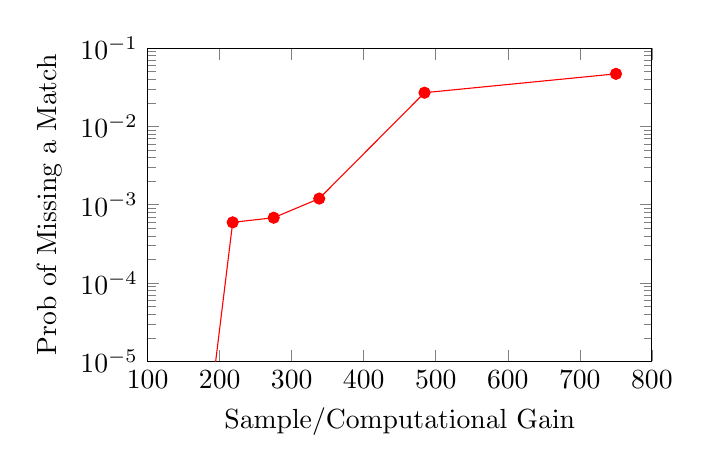
\begin{tikzpicture}

\begin{axis}[%
width=2.521in,
height=1.566in,
at={(0.758in,0.481in)},
scale only axis,
xmin=100,
xmax=800,
xlabel={Sample/Computational Gain},
ymode=log,
ymin=1e-05,
ymax=0.1,
yminorticks=true,
ylabel={Prob of Missing a Match},
axis background/.style={fill=white}
]
\addplot [color=red,solid,mark=*,mark options={solid},forget plot]
  table[row sep=crcr]{%
167.8088	1e-07\\
218.0519	0.0005965\\
274.9922	0.0006834\\
338.1745	0.0012\\
484.384	0.027\\
750.2035	0.047\\
};
\end{axis}
\end{tikzpicture}% }&
			\subfloat[$M=10^3(\mu=0.25),~ \tilde{N}=10^6, ~G=10^{6}$]{% This file was created by matlab2tikz.
%
%The latest updates can be retrieved from
%  http://www.mathworks.com/matlabcentral/fileexchange/22022-matlab2tikz-matlab2tikz
%where you can also make suggestions and rate matlab2tikz.
%
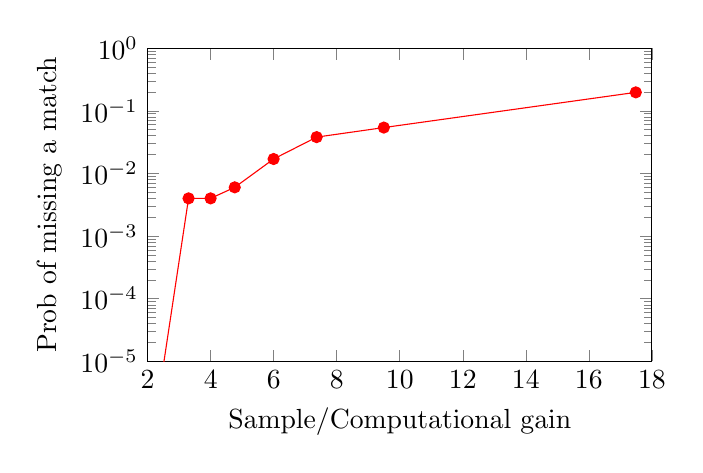
\begin{tikzpicture}

\begin{axis}[%
width=2.521in,
height=1.566in,
at={(0.758in,0.481in)},
scale only axis,
xmin=2,
xmax=18,
xlabel={Sample/Computational gain},
ymode=log,
ymin=1e-05,
ymax=1,
yminorticks=true,
ylabel={Prob of missing a match},
axis background/.style={fill=white}
]
\addplot [color=red,solid,mark=*,mark options={solid},forget plot]
  table[row sep=crcr]{%
2.0985	4e-07\\
3.2978	0.004\\
3.9974	0.004\\
4.7636	0.006\\
5.9963	0.017\\
7.3622	0.038\\
9.4944	0.054\\
17.4904	0.197\\
};
\end{axis}
\end{tikzpicture}% }
		\end{tabular}
		
		\caption{Plots of probability of missing a match vs. sample gain for exact matching of a query of length $M$ from a equiprobable  binary \{+1,-1\} sequence of length $N= 10^{12}$, divided into $G$ blocks each of length $\tilde{N}$. The substring was simulated to repeat in $L=10^6$($\lambda=0.5$) locations uniformly at random.} \label{Fig:Simulation Results}
\end{figure*}

Simulations were carried out to test the performance of RSIDFT framework for exact matching scenario on a database of length $N=10^{12}$ for two different query lengths $M=10^5$ ($\mu = 0.41$) and $M=10^3$ ($\mu = 0.25$). The database was generated as a equiprobable $\{+1,-1\}$ sequence of length $N$. A substring of length $M$ from the generated database is presented as a query. Also the chosen query was repeated at $L=10^6$ randomly chosen locations in the database.

The sample gain, defined as the ratio of $N$ to the number of samples used from the sketch of database, was varied and the probability of RSIDFT framework to miss a match ($P_e$), as defined below, was measured.
\[P_e = \frac{\text{\# of correctly identified locations}}{L} \]   
The plots of $P_e$ vs. sample gain, is presented in Fig.~\ref{Fig:Simulation Results} for two different query lengths: $M=10^5~(\mu=0.41)$ in Fig~\ref{Fig:Simulation Results}(a) and $M=10^3~(\mu=0.25)$ in Fig~\ref{Fig:Simulation Results}(b). As can be inferred from the plots we achieve a sample gain of 200-300 (depending on the tolerable error probability) for the query length corresponding to  $\mu=0.41$ and a sample gain of $2-4$ for $\mu=0.25$. This sample gain results from an average number of samples per branch $f_i \approx 9.2593e+07 $ ($\alpha=0.6639$) for $\mu=0.41$, and  $f_i \approx 6.9444e+09 $ ($\alpha=0.8201$) for $\mu=0.25$. The trend in the results almost matches with the theoretical findings of $\alpha = 1-\mu$. We also notice a sharp threshold in the sample gain below which the RSIDFT framework succeeds with very high probability.    		